%%%%%%%%%%%%%%%%%%%%%%%%%%%%%%%%%%%%%%%%%%%%%%%%%%%%%%
%%%%%%%%%%%%%%%%%%%%%%%%%%%%%%%%%%%%%%%%%%%%%%%%%%%%%%

\documentclass[xcolor=x11names,compress]{beamer}

\usepackage[backend=bibtex]{biblatex}
\bibliography{main}

\usepackage{appendixnumberbeamer}
\usepackage{amsmath}
\usepackage{graphicx}
\usepackage{palatino}

\useoutertheme[subsection=false,shadow]{miniframes}
\useinnertheme{default}
\usefonttheme{serif}

\setbeamerfont{title like}{shape=\scshape}
\setbeamerfont{frametitle}{shape=\scshape}

\setbeamercolor*{lower separation line head}{bg=DeepSkyBlue4}
\setbeamercolor*{normal text}{fg=black,bg=white}
\setbeamercolor*{alerted text}{fg=red}
\setbeamercolor*{example text}{fg=black}
\setbeamercolor*{structure}{fg=black}
\setbeamercolor*{palette tertiary}{fg=black,bg=black!10}
\setbeamercolor*{palette quaternary}{fg=black,bg=black!10}

\setbeamertemplate{caption}[numbered]

%%%%%%%%%%%%%%%%%%%%%%%%%%%%%%%%%%%%%%%%%%%%%%%%%%%%%%
%%%%%%%%%%%%%%%%%%%%%%%%%%%%%%%%%%%%%%%%%%%%%%%%%%%%%%

\begin{document}

\beamertemplatenavigationsymbolsempty

\title{The Development of Purdue's Computerized Interactive Teaching Assistant}
\subtitle{The CITA on CHIP Project}
\author{
    Presenter: Cyrus Vandrevala\\
    \vspace{3mm}
    Committee: Lynn Bryan, Andrew Hirsch,\\
    Hisao Nakanishi, and Laura Pyrak-Nolte\\
    \vspace{3mm}
    {\it Purdue University}\\
}
\date{August 30, 2016}

%%%%%%%%%%%%%%%%%%%%%%%%%%%%%%%%%%%%%%%%%%%%%%%%%%%%%%
%%%%%%%%%%%%%%%%%%%%%%%%%%%%%%%%%%%%%%%%%%%%%%%%%%%%%%

\begin{frame}
    \titlepage
\end{frame}

%%%%%%%%%%%%%%%%%%%%%%%%%%%%%%%%%%%%%%%%%%%%%%%%%%%%%%
%%%%%%%%%%%%%%%%%%%%%%%%%%%%%%%%%%%%%%%%%%%%%%%%%%%%%%

\begin{frame}{Table of Contents}
    \tableofcontents
\end{frame}

%%%%%%%%%%%%%%%%%%%%%%%%%%%%%%%%%%%%%%%%%%%%%%%%%%%%%%
%%%%%%%%%%%%%%%%%%%%%%%%%%%%%%%%%%%%%%%%%%%%%%%%%%%%%%

\section{\scshape Background}

\subsection{Electricity and Optics}

\begin{frame}{Electricity and Optics}
	\framesubtitle{PHYS 24100 and 24100D}
\end{frame}

\subsection{The CITA System}

\begin{frame}{CITA on CHIP}
\end{frame}

%%%%%%%%%%%%%%%%%%%%%%%%%%%%%%%%%%%%%%%%%%%%%%%%%%%%%%
%%%%%%%%%%%%%%%%%%%%%%%%%%%%%%%%%%%%%%%%%%%%%%%%%%%%%%

\section{\scshape Methodology}

\subsection{Schedule of Development and Analysis}

\begin{frame}{Schedule of Development}
	\begin{table}[ht]
		\caption{In the spring semester of 2015 (and before), the CHIP homework system included 29 ``interactive examples'' that were originally developed by the faculty at UIUC (out of 139 homework problems total).}
		\begin{center}
			\begin{tabular}{|c|c|c|}
				\hline
				\textbf{Semester} & \textbf{Section} & \textbf{Version}\\
				\hline
				Spring 2015 and Before & Campus & Pre-CITA\\
				& Online & Pre-CITA\\
				\hline
				Summer 2015 & Online & 1.0 (Beta)\\
				\hline
				Fall 2015 & Campus & 2.0\\
				& Online & 1.0 (Beta)\\
				\hline
				Spring 2016 & Campus & 3.0\\
				& Online & 3.0\\
				\hline
				Summer 2016 & Online & 3.0\\
				\hline
			\end{tabular}
		\end{center}
		\label{tab:schedule}
	\end{table}
\end{frame}

\begin{frame}{Schedule of Analysis}
	We employed the sequential exploratory strategy since it is useful for the development and testing of a new instrument. One repeats phases of qualitative data analysis followed by phases of quantitative data analysis\footfullcite{creswell2003}.
	\vspace{3mm}
	\begin{enumerate}
		\item The project started with an analysis of student comments along with a literature review.
		\item We collected quantitative data during the semester and qualitative data at the end of the semester.
		\item We analyzed one type of data while collecting the other.
		\item We performed a final recap analysis in the summer of 2016.
	\end{enumerate}
\end{frame}

\subsection{Qualitative Procedures}

\begin{frame}{Strategy of Inquiry}
	Qualitative data for this project came from three major sources:
	\vspace{1mm}
	\begin{itemize}
		\item Final Question from Exit Survey
		\item Piazza Comments
		\item Focus Group Sessions
	\end{itemize}
	\vspace{5mm}
	We analyzed the data using a three-cycle coding plan\footfullcite{saldana2012}:
	\vspace{1mm}
	\begin{itemize}
		\item \textbf{First Cycle:} Attribute and Descriptive Coding
		\item \textbf{Second Cycle:} Elaborative and Pattern Coding
		\item \textbf{Third Cycle:} Evaluation and Longitudinal Coding
	\end{itemize}
\end{frame}

\begin{frame}{Focus Group Sessions}
	Focus group sessions were used for a variety of reasons\footfullcite{hennink2014}:
	\vspace{1mm}
	\begin{itemize}
		\item Exploratory, explanatory, and evaluative research
		\item Large amounts of data with a range of viewpoints
		\item Limits researcher influence
	\end{itemize}
	\vspace{5mm}
	We used purposeful sampling as our design strategy\footfullcite{patton2015}:
	\vspace{1mm}
	\begin{itemize}
		\item Overall Impression of the Homework System
		\item Online vs. On-Campus Section of the Class
	\end{itemize}
\end{frame}

\begin{frame}{Roles of the Researchers}
	\begin{itemize}
		\item \textbf{Cyrus Vandrevala:} Teaching Assistant, Course Coordinator, Developed Online Course, Developed CITA Tutorials, Led Focus Group Sessions, Data Analysis
		\vspace{2mm}
		\item \textbf{Hisao Nakanishi:} Helped Develop CHIP and CITA, Scheduled Assignments, Answered Student Questions Through CHIP, Data Analysis
		\vspace{2mm}
		\item \textbf{Laura Pyrak-Nolte:} Course Administrator, Course Instructor, Lecturer for Online Sections, Data Analysis
		\vspace{2mm}
		\item \textbf{Lynn Bryan:} Theoretical Background
		\vspace{2mm}
		\item \textbf{Andrew Hirsch:} Instructor for PHYS 17200
		\vspace{2mm}
		\item \textbf{Gary Johns:} Teaching Assistant (24100 and 17200), Data Analysis
	\end{itemize}
\end{frame}

%%%%%%%%%%%%%%%%%%%%%%%%%%%%%%%%%%%%%%%%%%%%%%%%%%%%%%
%%%%%%%%%%%%%%%%%%%%%%%%%%%%%%%%%%%%%%%%%%%%%%%%%%%%%%

\section{\scshape Results}

\subsection{Student Motivations}

\begin{frame}{Efficiency}
	More than anything else, students are interested in completing the homework as quickly and efficiently as possible.
\end{frame}

%%%%%%%%%%%%%%%%%%%%%%%%%%%%%%%%%%%%%%%%%%%%%%%%%%%%%%
%%%%%%%%%%%%%%%%%%%%%%%%%%%%%%%%%%%%%%%%%%%%%%%%%%%%%%

\section{\scshape Conclusions}

\subsection{Summary}
\begin{frame}{Summary}
    \begin{itemize}
        \item We paired a number of tutorials with homework problems
        \item Thematic Analysis of Online Homework Systems
        \item Cupcake Physics
    \end{itemize}
\end{frame}

\subsection{Future Directions}
\begin{frame}{Future Directions}
    \begin{itemize}
        \item At Purdue
        \begin{itemize}
            \item Write Up Piazza Results
            \item Thematic Analysis of Online Homework Systems
        \end{itemize}
        \vspace{3mm}
        \item For Me Personally
        \begin{itemize}
            \item Cupcake Physics
        \end{itemize}
    \end{itemize}
\end{frame}

%%%%%%%%%%%%%%%%%%%%%%%%%%%%%%%%%%%%%%%%%%%%%%%%%%%%%%
%%%%%%%%%%%%%%%%%%%%%%%%%%%%%%%%%%%%%%%%%%%%%%%%%%%%%%

\appendix
\section{\scshape Backup Slides}

\subsection{Relationship Between P-Value and $R^2$}

\begin{frame}{Relationship Between P-Value and $R^2$}
	\begin{itemize}
		\item \textit{Large P, Large $R^2$:}\newline
		Data appears linear because there are few data points.
		\vspace{2mm}
		\item \textit{Large P, Small (or Negative) $R^2$:}\newline
		Data does not follow a linear model at all.
		\vspace{2mm}
		\item \textit{Small P, Large $R^2$:}\newline
		Data follows a linear model with a good fit.
		\vspace{2mm}
		\item \textit{Small P, Small $R^2$:}\newline
		Data follows a linear model, but the range of the data is large.
	\end{itemize}
\end{frame}

\subsection{Overall Grade vs. Number of Clicks for AP Physics Students}

\begin{frame}{Overall Grade vs. Number of Clicks}
	\framesubtitle{AP Physics Students}
	\begin{figure}
		\centering
		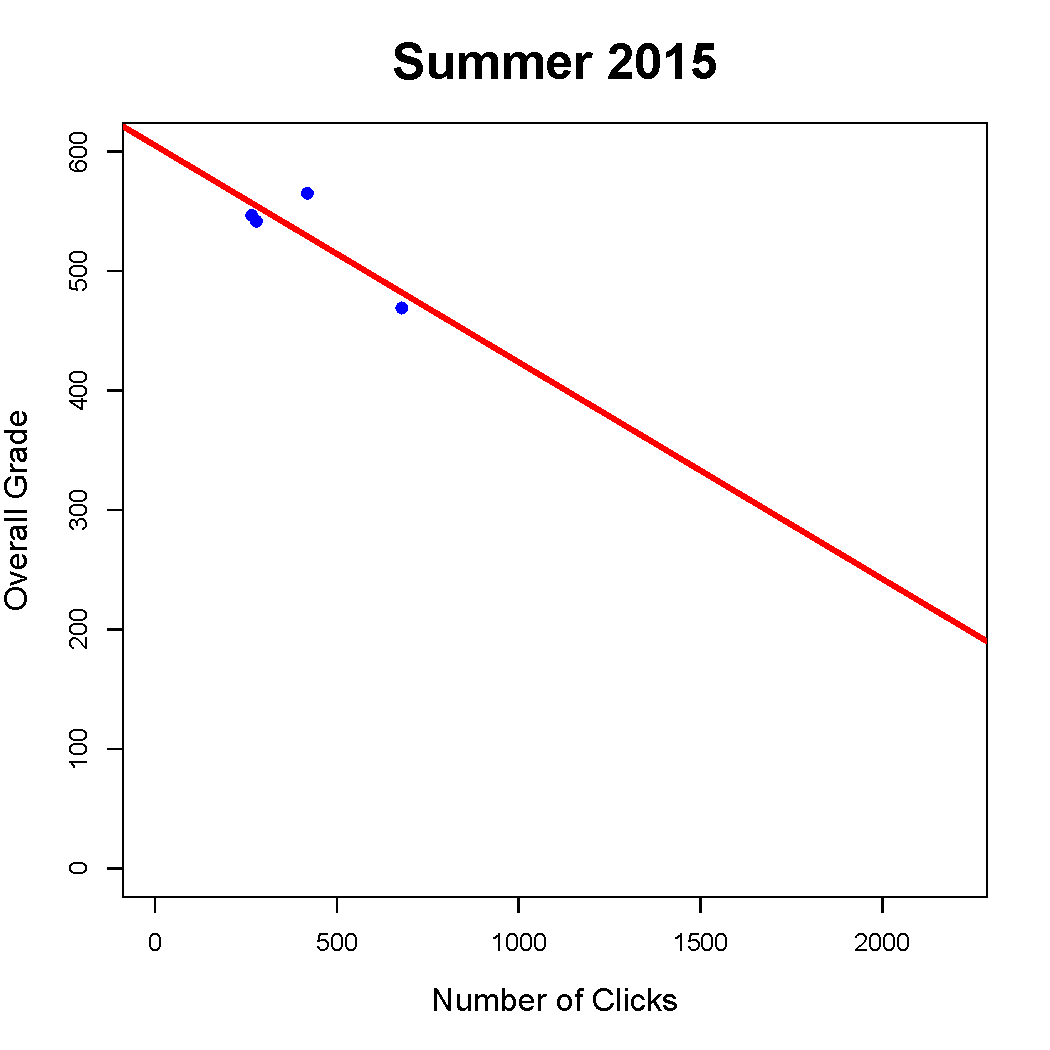
\includegraphics[width=0.33\textwidth]{img/overall_grade_vs_clicks_su15_ap_students.pdf}
		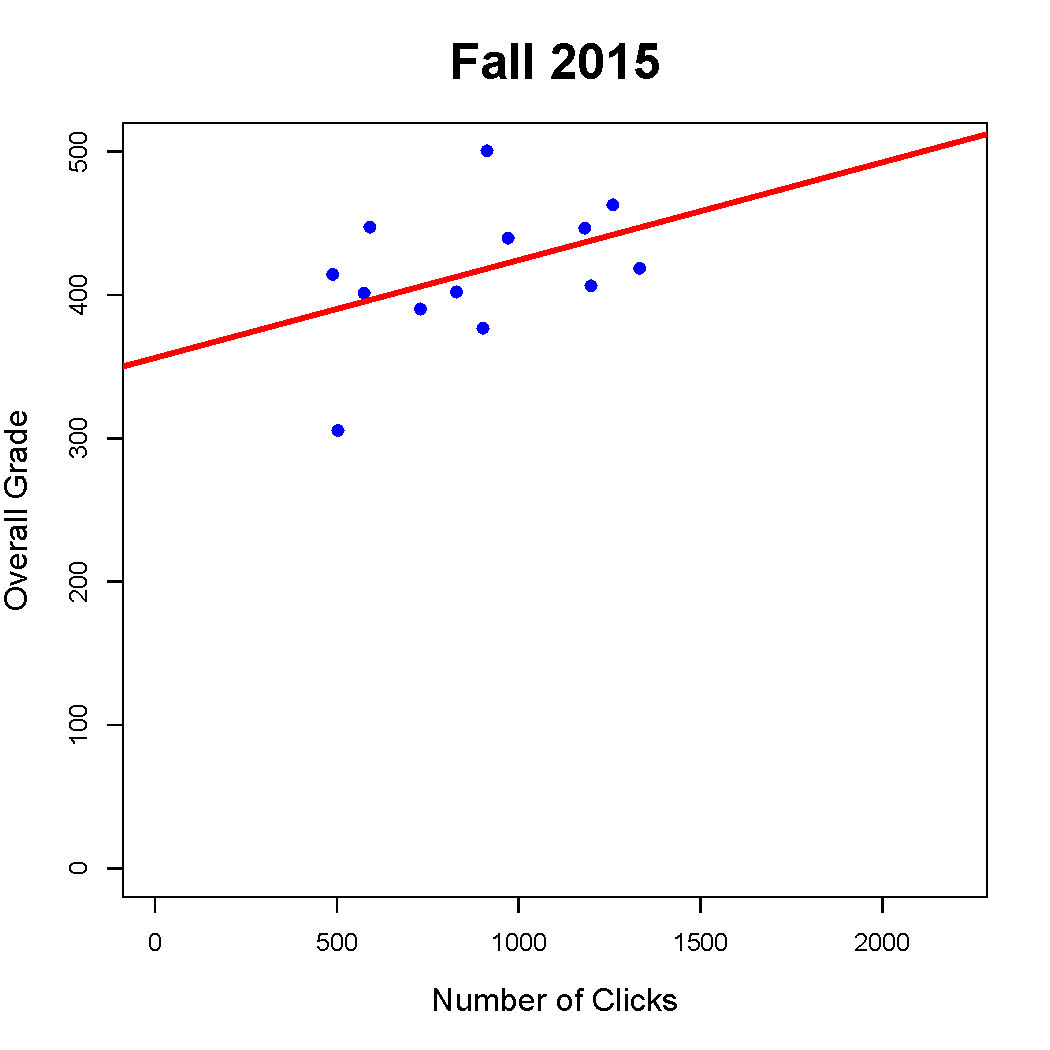
\includegraphics[width=0.33\textwidth]{img/overall_grade_vs_clicks_fa15_ap_students.pdf}
		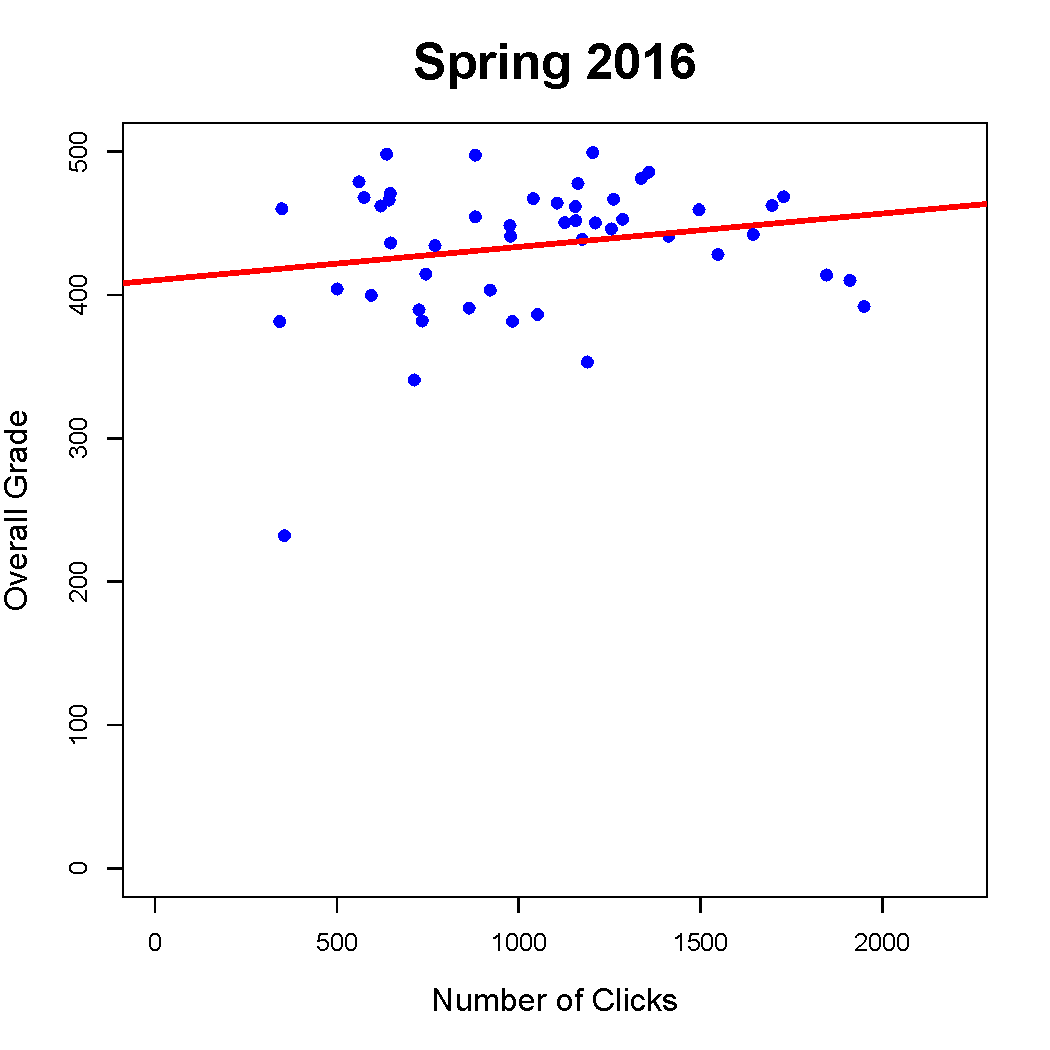
\includegraphics[width=0.33\textwidth]{img/overall_grade_vs_clicks_sp16_ap_students.pdf}
		\caption{In the summer and fall of 2015, a linear model did not fit the data due to the small sample sizes ($p = 0.177$ and $p = 0.146$, respectively). In the spring of 2016, a linear model did not fit the data due to the large range of Overall Grades ($p = 0.165$).}
		\label{fig:overall_grade_vs_clicks_ap_students}
	\end{figure}
\end{frame}

%%%%%%%%%%%%%%%%%%%%%%%%%%%%%%%%%%%%%%%%%%%%%%%%%%%%%%
%%%%%%%%%%%%%%%%%%%%%%%%%%%%%%%%%%%%%%%%%%%%%%%%%%%%%%

\end{document}
